\begin{frame}[fragile]{Chisel has a Multiplexer}
\begin{figure}
  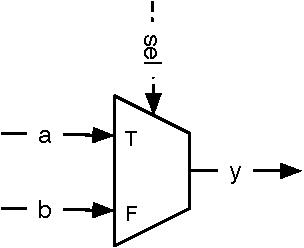
\includegraphics[scale=\scale]{../figures/mux}
\end{figure}
\shortlist{../code/mux.txt}
\begin{itemize}
\item So what?
\item Wait... What type is \code{a} and \code{b}?
\begin{itemize}
\item Can be any Chisel type!
\end{itemize}
\end{itemize}
\end{frame}

\begin{frame}[fragile]{Chisel has a Generic Multiplexer}
\begin{figure}
  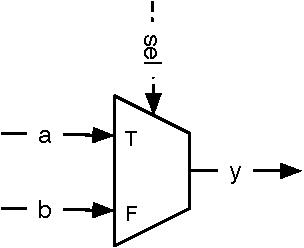
\includegraphics[scale=\scale]{../figures/mux}
\end{figure}
\shortlist{../code/mux.txt}
\begin{itemize}
\item SW people may not be impressed
\item They have generics since Java 1.5 in 2004
\begin{itemize}
\item \code{List<Flowers> != List<Cars>}
\end{itemize}
\end{itemize}
\end{frame}


\begin{frame}[fragile]{Generics in Hardware Construction}
\begin{itemize}
\item Chisel supports generic classes with type parameters
\item Write hardware generators independent of concrete type
\item This is a multiplexer \emph{generator}
\end{itemize}
\shortlist{../code/param_func.txt}
\end{frame}

\begin{frame}[fragile]{Put Generics Into Use}
\begin{itemize}
\item Let us implement a generic FIFO
\item Use the generic ready/valid interface from Chisel
\end{itemize}
\shortlist{../code/fifo_decoupled.txt}
\end{frame}

\begin{frame}[fragile]{Define the FIFO Interface}
\shortlist{../code/fifo_io.txt}
\begin{itemize}
\item We need enqueueing and dequeueing ports
\item Note the \code{Flipped}
\begin{itemize}
\item It switches the direction of ports
\item No more double definitions of an interface
\end{itemize}
\end{itemize}
\end{frame}

\begin{frame}[fragile]{But What FIFO Implementation?}
\begin{itemize}
\item Bubble FIFO (good for low data rate)
\item Double buffer FIFO (fast restart)
\item FIFO with memory and pointers (for larger buffers)
\begin{itemize}
\item Using flip-flops
\item Using on-chip memory
\end{itemize}
\item And some more...
\end{itemize}
\begin{itemize}
\item This calls for object-oriented \sout{programming} \emph{hardware construction}
\end{itemize}
\end{frame}

\begin{frame}[fragile]{Abstract Base Class and Concrete Extension}
\shortlist{../code/fifo_abstract.txt}
\begin{itemize}
\item May contain common code
\item Extend by concrete classes
\end{itemize}
\begin{chisel}
class BubbleFifo[T <: Data](gen: T, depth: Int) extends Fifo(gen: T, depth: Int) {
\end{chisel}
\end{frame}



\begin{frame}[fragile]{Select a Concrete FIFO Implementation}
\begin{itemize}
\item Decide at hardware generation
\item Can use all Scala/Java power for the decision
\begin{itemize}
\item Connect to a web service, get \sout{Google} Alphabet stock price, and decide on which to use ;-)
\item For sure a silly idea, but you see what is possible...
\item Developers may find clever use of the Scala/Java power
\item We could present a GUI to the user to select from
\end{itemize}
\item We use XML files parsed at hardware generation time
\item End of TCL, Python,... generated hardware
\end{itemize}
\end{frame}

\begin{frame}[fragile]{Binary to BCD Conversion for VHDL}
\begin{figure}
    \centering
    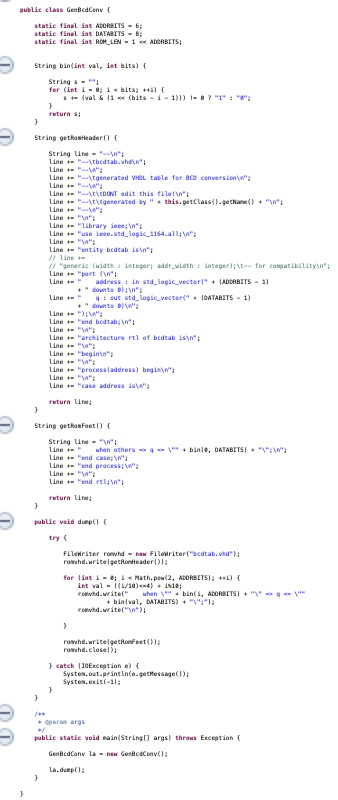
\includegraphics[scale=0.6]{JavaBCD}
\end{figure}
\end{frame}

\begin{frame}[fragile]{Java Program}
\begin{itemize}
\item Generates a VHDL table
\item The core code is:
\end{itemize}
\begin{chisel}
for (int i = 0; i < Math.pow(2, ADDRBITS); ++i) {
    int val = ((i/10)<<4) + i%10;
    // write out VHDL code for each line
\end{chisel}
\begin{itemize}
\item With all boilerplate 118 LoC
\end{itemize}
\end{frame}

\begin{frame}[fragile]{Chisel Version of Binary to BCD Conversion}
%\begin{chisel}
%  val array = new Array[Int](256)
%  for (i <- 0 to 99) {
%    array(i) = ((i/10)<<4) + i%10
%  }
%  val table = VecInit(array.map(_.U(8.W)))
%\end{chisel}
\begin{chisel}
  val table = Wire(Vec(100, UInt(8.W)))
  for (i <- 0 until 100) {
    table(i) := (((i/10)<<4) + i%10).U
  }
  val bcd = table(bin)
\end{chisel}
\begin{itemize}
\item Directly generates the hardware table as a \code{Vec}
\item At hardware construction time
\item In the same language
\end{itemize}
\end{frame}

\begin{frame}[fragile]{Use Functional Programming for Generators}
\shortlist{../code/fun_first.txt}
\shortlist{../code/fun_func_lit.txt}
\shortlist{../code/fun_reduce_tree.txt}
\begin{itemize}
\item This is a simple example
\item What about an arbitration tree with fair arbitration?
\end{itemize}
\end{frame}

\begin{frame}[fragile]{Functional Generation}
\begin{itemize}
\item Anonymous functions, called \emph{function literal}
\begin{chisel}
  (param) => function body
\end{chisel}
\item A function for a minimum search
\shortlist{../code/fun_min.txt}
\end{itemize}
\end{frame}

\begin{frame}[fragile]{Minimal Function with Index}
\begin{itemize}
\item Was the example for Tjark's heap sort
\shortlist{../code/fun_min2.txt}
\item We need an extra bundle to hold both values
\item A for loop is not so functional
\end{itemize}
\end{frame}

\begin{frame}[fragile]{We Can Use Tuples and zipWithIndex}
\begin{itemize}
\item \code{zipWithIndex} transforms the original sequence to a sequence of tuples
with second element is the index
\item Use \code{map} to translate from Scala \code{Int} to Chisel \code{UInt}
\item \code{reduce} does the minimum function, actually called 2 times (we could optimize this)
\shortlist{../code/fun_min3.txt}
\item The result is a Scala \code{Vector} and not a Chisel \code{Vec}
\end{itemize}
\end{frame}

\begin{frame}[fragile]{Solution with a Vec}
\begin{itemize}
\item This results in a Chisel \code{Vec}
\shortlist{../code/fun_min4.txt}
\item
\item We should add a \code{reduceTree} to the Scala sequence version (\code{TraversableOnce})
\end{itemize}
\end{frame}

%\begin{frame}[fragile]{An Arbiter}
%\shortlist{../code/fun_arbiter.txt}
%\end{frame}
%
%
%
%\begin{frame}[fragile]{XXX}
%\begin{itemize}
%\item TODO: s4noc connection is part of the generator story
%\item
%\item
%\end{itemize}
%\end{frame}
%
%\begin{frame}[fragile]{XXX}
%\begin{itemize}
%\item
%\item
%\item
%\end{itemize}
%\end{frame}

